% ŠABLONA PRO PSANÍ ZÁVĚREČNÉ STUDIJNÍ PRÁCE
%%%%%%%%%%%%%%%%%%%%%%%%%%%%%%%%%%%%%%%%%%%%
% Autor: Jakub Dokulil (kubadokulil99@gmail.com)
% Tato šablona byla vytvořena tak, aby pomocí ní mohli v systému LaTeX soutěžící sázet své práce a zároveň odpovídala požadavkům na formátování vyplývajícím z wordové šablony umístěné na webu soc.cz.
%
\documentclass[12pt,a4paper,twoside,openany]{report}
%oneside,      %% -- odkomentujte, pokud chcete svou práci mít pouze jednostrannou, mezera pro hřbet pak automaticky bude pouze na levé straně



% --- odstraneni zbytkoveho textu "superiorSup" a pod. ---
\AtBeginDocument{%
	% pojistka proti nechtenemu textu nactenemu z aux/toc
	\immediate\write16{(cleaning stray figureversions output...)}%
	\clearpage
	\thispagestyle{empty}
	% uplne vyprazdneni vseho, co by se objevilo mimo hlavni text
	\let\superiorSup\relax
	\let\textOsF\relax
	\let\textTOsF\relax
	\let\liningLF\relax
	\let\liningTLF\relax
	\let\tabularTab\relax
	\let\proportionalProp\relax
	\let\tabularmath\relax
	\let\proportionalmath\relax
	\let\fontspechyperref\relax
	% zajisteni, ze se nic nezobrazi pred titulni stranou
	\null
	\newpage
}
%% Nutné balíčky a nastavení
%%%%%%%%%%%%%%%%%%%%%%%%%%%%

%% Proměnné
\newcommand\obor{INFORMAČNÍ TECHNOLOGIE} %% -- napiš číslo a název tvého oboru
\newcommand\kodOboru{18-20-M/01} %% -- napiš číslo a název tvého oboru
\newcommand\zamereni{se zaměřením na počítačové sítě a programování} %% -- napiš číslo a název tvého oboru
\newcommand\skola{Střední škola průmyslová a umělecká, Opava} %% vyplň název školy
\newcommand\trida{IT4} %% vyplň jméno svého konzultanta
\newcommand\jmenoAutora{Denis Adamčík}  %% vyplň své jméno
\newcommand\skolniRok{2025/26} %% vyplň rok
\newcommand\datumOdevzdani{1. 1. 2026} %% vyplň rok
\newcommand\nazevPrace{Auto na dálkové ovládání} %% vyplň název své práce

\title{\nazevPrace} %% -- Název tvé práce
\author{\jmenoAutora} %% -- tvé jméno
\date{\datumOdevzdani} %% -- rok, kdy píšeš SOČku

\usepackage[top=2.5cm, bottom=2.5cm, left=3.5cm, right=1.5cm]{geometry} %% nastaví okraje, left -- vnitřní okraj, right -- vnější okraj

\usepackage[czech]{babel} %% balík babel pro sazbu v češtině
\usepackage[utf8]{inputenc} %% balíky pro kódování textu
\usepackage[T1]{fontenc}
\usepackage{cmap} %% balíček zajišťující, že vytvořené PDF bude prohledávatelné a kopírovatelné

\usepackage{graphicx} %% balík pro vkládání obrázků

\usepackage{subcaption} %% balíček pro vkládání podobrázků

\usepackage{hyperref} %% balíček, který v PDF vytváří odkazy
\usepackage{float}
\usepackage{expl3}
\linespread{1.25} %% řádkování
\setlength{\parskip}{0.5em} %% odsazení mezi odstavci


\usepackage[pagestyles]{titlesec} %% balíček pro úpravu stylu kapitol a sekcí
\titleformat{\chapter}[block]{\scshape\bfseries\LARGE}{\thechapter}{10pt}{\vspace{0pt}}[\vspace{-22pt}]
\titleformat{\section}[block]{\scshape\bfseries\Large}{\thesection}{10pt}{\vspace{0pt}}
\titleformat{\subsection}[block]{\bfseries\large}{\thesubsection}{10pt}{\vspace{0pt}}


\usepackage{tocloft} % Balíček umožní přizpůsobit vzhled tabulky obsahu
\setlength{\cftbeforechapskip}{0pt}  % Menší rozestup pro kapitoly
\setlength{\cftbeforesecskip}{0pt}   % Menší rozestup pro sekce

\setcounter{secnumdepth}{2}
\setcounter{tocdepth}{1}
\usepackage{fancyhdr}
\pagestyle{fancy}
\renewcommand{\headrulewidth}{0.025pt}

\usepackage{booktabs}

\usepackage{url}

%% Balíčky co se můžou hodit :) 
%%%%%%%%%%%%%%%%%%%%%%%%%%%%%%%

\usepackage{pdfpages} %% Balíček umožňující vkládat stránky z PDF souborů, 

\usepackage{upgreek} %% Balíček pro sazbu stojatých řeckých písmen, třeba u jednotky mikrometr. Například stojaté mí: \upmu, stojaté pí: \uppi

\usepackage{amsmath}    %% Balíčky amsmath a amsfonts 
\usepackage{amsfonts}   %% pro sazbu matematických symbolů
\usepackage{esint}     %% pro sazbu různých integrálů (např \oiint)
\usepackage{mathrsfs}
\usepackage{helvet} % Helvet font
\usepackage{mathptmx} % Times New Roman
\makeatletter
\@namedef{ver@figureversions.sty}{9999/99/99}
\newcommand{\DeclareFigureVersion}[2]{}
\newcommand{\figureversion}[1]{}
\makeatother


\makeatletter
\providecommand{\superiorSup}{}
\providecommand{\textOsF}{}
\providecommand{\textTOsF}{}
\providecommand{\liningLF}{}
\providecommand{\liningTLF}{}
\providecommand{\tabularTab}{}
\providecommand{\proportionalProp}{}
\makeatother
\makeatletter
\providecommand{\superiorSup}{}
\providecommand{\textOsF}{}
\providecommand{\textTOsF}{}
\providecommand{\liningLF}{}
\providecommand{\liningTLF}{}
\providecommand{\tabularTab}{}
\providecommand{\proportionalProp}{}
\providecommand{\tabularmath}{}
\providecommand{\proportionalmath}{}
\makeatother

%%\usepackage{Oswald} % Oswald font


%% makra pro sazbu matematiky
\newcommand{\dif}{\mathrm{d}} %% makro pro sazbu diferenciálu, místo toho
%% abych musel psát '\mathrm{d}' mi stačí napsat '\dif' což je mnohem 
%% kratší a mohu si tak usnadnit práci

\usepackage{listings}
\usepackage{xcolor}

\renewcommand{\lstlistingname}{Kód}% Listing -> Algorithm
\renewcommand{\lstlistlistingname}{Seznam programových kódů}% List of Listings -> List of Algorithms

%% Definice 
\lstdefinelanguage{JavaScript}{
	morekeywords=[1]{break, continue, delete, else, for, function, if, in,
		new, return, this, typeof, var, void, while, with},
	% Literals, primitive types, and reference types.
	morekeywords=[2]{false, null, true, boolean, number, undefined,
		Array, Boolean, Date, Math, Number, String, Object},
	% Built-ins.
	morekeywords=[3]{eval, parseInt, parseFloat, escape, unescape},
	sensitive,
	morecomment=[s]{/*}{*/},
	morecomment=[l]//,
	morecomment=[s]{/**}{*/}, % JavaDoc style comments
	morestring=[b]',
	morestring=[b]"
}[keywords, comments, strings]


\lstdefinelanguage[ECMAScript2015]{JavaScript}[]{JavaScript}{
	morekeywords=[1]{await, async, case, catch, class, const, default, do,
		enum, export, extends, finally, from, implements, import, instanceof,
		let, static, super, switch, throw, try},
	morestring=[b]` % Interpolation strings.
}

\lstalias[]{ES6}[ECMAScript2015]{JavaScript}

% Nastavení barev
% Requires package: color.
\definecolor{mediumgray}{rgb}{0.3, 0.4, 0.4}
\definecolor{mediumblue}{rgb}{0.0, 0.0, 0.8}
\definecolor{forestgreen}{rgb}{0.13, 0.55, 0.13}
\definecolor{darkviolet}{rgb}{0.58, 0.0, 0.83}
\definecolor{royalblue}{rgb}{0.25, 0.41, 0.88}
\definecolor{crimson}{rgb}{0.86, 0.8, 0.24}

% Nastavení pro Python
\lstdefinestyle{Python}{
	language=Python,
	backgroundcolor=\color{white},
	basicstyle=\ttfamily,
	breakatwhitespace=false,
	breaklines=false,
	captionpos=b,
	columns=fullflexible,
	commentstyle=\color{mediumgray}\upshape,
	emph={},
	emphstyle=\color{crimson},
	extendedchars=true,  % requires inputenc
	fontadjust=true,
	frame=single,
	identifierstyle=\color{black},
	keepspaces=true,
	keywordstyle=\color{mediumblue},
	keywordstyle={[2]\color{darkviolet}},
	keywordstyle={[3]\color{royalblue}},
	literate=%
	{á}{{\'a}}1 {č}{{\v{c}}}1 {ď}{{\v{d}}}1 {é}{{\'e}}1 {ě}{{\v{e}}}1
	{í}{{\'i}}1 {ň}{{\v{n}}}1 {ó}{{\'o}}1 {ř}{{\v{r}}}1 {š}{{\v{s}}}1
	{ť}{{\v{t}}}1 {ú}{{\'u}}1 {ů}{{\r{u}}}1 {ý}{{\'y}}1 {ž}{{\v{z}}}1,		
	numbers=left,
	numbersep=5pt,
	numberstyle=\tiny\color{black},
	rulecolor=\color{black},
	showlines=true,
	showspaces=false,
	showstringspaces=false,
	showtabs=false,
	stringstyle=\color{forestgreen},
	tabsize=2,
	title=\lstname,
	upquote=true  % requires textcomp	
}


\lstdefinestyle{JSES6Base}{
	backgroundcolor=\color{white},
	basicstyle=\ttfamily,
	breakatwhitespace=false,
	breaklines=false,
	captionpos=b,
	columns=fullflexible,
	commentstyle=\color{mediumgray}\upshape,
	emph={},
	emphstyle=\color{crimson},
	extendedchars=true,  % requires inputenc
	fontadjust=true,
	frame=single,
	identifierstyle=\color{black},
	keepspaces=true,
	keywordstyle=\color{mediumblue},
	keywordstyle={[2]\color{darkviolet}},
	keywordstyle={[3]\color{royalblue}},
 literate=%
{á}{{\'a}}1 {č}{{\v{c}}}1 {ď}{{\v{d}}}1 {é}{{\'e}}1 {ě}{{\v{e}}}1
{í}{{\'i}}1 {ň}{{\v{n}}}1 {ó}{{\'o}}1 {ř}{{\v{r}}}1 {š}{{\v{s}}}1
{ť}{{\v{t}}}1 {ú}{{\'u}}1 {ů}{{\r{u}}}1 {ý}{{\'y}}1 {ž}{{\v{z}}}1,		
	numbers=left,
	numbersep=5pt,
	numberstyle=\tiny\color{black},
	rulecolor=\color{black},
	showlines=true,
	showspaces=false,
	showstringspaces=false,
	showtabs=false,
	stringstyle=\color{forestgreen},
	tabsize=2,
	title=\lstname,
	upquote=true  % requires textcomp
}

\lstdefinestyle{JavaScript}{
	language=JavaScript,
	style=JSES6Base,
}
\lstdefinestyle{ES6}{
	language=ES6,
	style=JSES6Base
}

\setlength{\headheight}{15pt}

%% Bordel pro práci - můžeš smáznout :) 
%%%%%%%%%%%%%%%%%%%

\usepackage{lipsum} %% balíček který píše lipsum (nesmyslný text, který se používá pro kontrolu typografie)

\AtBeginDocument{\clearpage\pagestyle{empty}}

%% Začátek dokumentu
%%%%%%%%%%%%%%%%%%%%
\begin{document}
	
	\pagestyle{empty}
	\pagenumbering{Roman}
	
	\cleardoublepage

%% Titulní stránka s informacemi
%%%%%%%%%%%%%%%%%%%%%%%%%%%%%%%%%%%%%%%%
	
	{\fontfamily{phv}\selectfont
		%% Logo školy
		\begin{figure}[h]
			\centering
			\includegraphics[width=0.6\linewidth]{image/logo-skoly.png} 
		\end{figure}
		
		
		%% Hlavička práce a její název (viz proměnná \nazev prace)
		%% \sffamily %%% bezpatkové písmo - sans serif
		{\bfseries %%% písmo na stránce je tučně
			\begin{center}
				\vspace{0.025 \textheight}
				\LARGE{ZÁVĚREČNÁ STUDIJNÍ PRÁCE}\\
				\large{dokumentace}\\
				\vspace{0.075 \textheight}
				\LARGE {\nazevPrace}\\
			\end{center}  
		}%%%
		
		\begin{figure}[h]
			\centering
			\includegraphics[width=0.8\linewidth]{image/programovani-02.jpg} 
		\end{figure}
		
		\vspace{0.02 \textheight}
		\begin{table}[h!]
			\begin{tabular}{ll}
				\textbf{Autor:} & \jmenoAutora\\ 
				\textbf{Obor:} & \kodOboru { } \obor\\
				\textbf{} & \zamereni\\
				\textbf{Třída:} & \trida\\
				\textbf{Školní rok:} & \skolniRok\\
			\end{tabular}
			
		\end{table}		
	}
	
\cleardoublepage %% Zalomení dvojstránky
	
%% Stránka obsahující poděkování a prohlášení
%%%%%%%%%%%%%%%%%%%%%%%%%%%%%%%%%%%%%%%%%%%%%%%%%%%%%%%%

%% Poděkování - nepovinné
%%%%%%%%%%%%%%%%%%%%%%%%%%%%
	
	\noindent{\large{\bfseries{Poděkování}\\}}
	\noindent Rád bych podekoval panu učiteli Mgr. Marcelu Godovskému za nápady a součástky potřebné k projektu.
	
	\vspace*{0.7\textheight} %% Vertikální mezeru je možné upravit

%% Prohlášení - povinné
%%%%%%%%%%%%%%%%%%%%%%%%%%%%
	\noindent{\large{\bfseries{Prohlášení}\\}}  %% uprav si koncovky podle toho na jaký rod se cítíš, vypadá to pak lépe :) 
	\noindent{Prohlašuji, že jsem závěrečnou práci vypracoval samostatně a uvedl veškeré použité 
		informační zdroje.\\}
	\noindent{Souhlasím, aby tato studijní práce byla použita k výukovým a prezentačním účelům na Střední průmyslové a umělecké škole v Opavě, Praskova 399/8.}
	\vfill
	\noindent{V Opavě \datumOdevzdani\\}
	\noindent
	\begin{minipage}{\linewidth}
		\hspace{9.5cm} 
		\begin{tabular}{@{}p{6cm}@{}}
			\dotfill \\
			Podpis autora
		\end{tabular}
	\end{minipage}
	

%% Stránka obsahující abstrakt (anotaci)
%%%%%%%%%%%%%%%%%%%%%%%%%%%%%%%%%%%%%%%%%%%%%%%%%%%%%%%%	

%% Abstrakt v češtině
%%%%%%%%%%%%%%%%%%%%%%%%%%%%
	\noindent{\Large{\bfseries{Abstrakt}\\}}
Tento ročníkový projekt popisuje návrh a realizaci RC autíčka ovládaného na dálku pomocí Wi-Fi, postaveného na mikrokontrolérech ESP8266. Projekt se skládá ze dvou částí: ovladače, který pomocí tlačítek generuje příkazy, a přijímače v autíčku, který přijímá tyto příkazy a převádí je na signály pro řízení dvou DC motorů přes H-můstky. Komunikace mezi ovladačem a autíčkem je realizována přes Wi-Fi protokol ESP-NOW, což umožňuje bezdrátové ovládání bez potřeby klasické sítě. Cílem projektu bylo demonstrovat základní principy bezdrátové komunikace, řízení pohybu a implementace jednoduchého dálkového ovládání v embedded systému.
	
	\vspace{18pt}
	
	\noindent{\large{\bfseries{Klíčová slova}}}
	
	\noindent Esp8266, ESP-NOW, modelování, sestavení, \dots 
	
	\vspace{18pt}

%% Abstrakt v angličtině
%%%%%%%%%%%%%%%%%%%%%%%%%%%%	
	\noindent{\Large{\bfseries{Abstract}}}
	
This year-end project presents the design and implementation of a Wi-Fi remote-controlled car, based on ESP8266 microcontrollers. The system consists of two main components: a controller, which sends button-driven commands, and a receiver installed on the car, which interprets these commands and converts them into control signals for two DC motors using H-bridge drivers. The communication between the controller and the car is carried out via the ESP-NOW Wi-Fi protocol, enabling wireless operation without a traditional network infrastructure. The aim of the project is to demonstrate fundamental concepts of wireless communication, motion control, and remote operation in an embedded system. 

	\vspace{18pt}
	
	\noindent{\large{\bfseries{Keywords}}}
	
	\noindent Esp8266, ESP-NOW, modeling, assembling  \dots 
	
	\clearpage %% Zalomení stránky

%% Stránka s generovaným obsahem
%%%%%%%%%%%%%%%%%%%%%%%%%%%%%%%%%%%%%%%	
	
	\tableofcontents %% Vygeneruje tabulku s obsahem

	\pagenumbering{arabic} %% Nastavení způsobu číslování stránek (alternativy roman | Roman)
	\setcounter{page}{1} %% Nastavení počitadla stránek

%% Stránka s úvodem - povinná část
%%%%%%%%%%%%%%%%%%%%%%%%%%%%%%%%%%%%%%%		
	\chapter*{Úvod}
%Tento příkaz vytvoří novou kapitolu s názvem "Úvod" ve vašem dokumentu.
%Hvězdička * u příkazu \chapter* znamená, že tato kapitola nebude mít číslo. Ve výsledném dokumentu se tedy objeví jako "Úvod" bez předcházejícího čísla kapitoly, které se obvykle zobrazuje u číslovaných kapitol.
%Tento příkaz také znamená, že kapitola se automaticky neobjeví v obsahu, protože LaTeX standardně zahrnuje do obsahu pouze číslované kapitoly.
	\addcontentsline{toc}{chapter}{Úvod}
%Tento příkaz ručně přidává záznam do obsahu.
%První parametr toc označuje, že přidáváme záznam do Table of Contents (obsahu).
%Druhý parametr chapter specifikuje úroveň záznamu. V tomto případě říkáme, že přidávaný záznam má být považován za kapitolu.
%Třetí parametr Úvod je text, který se objeví v obsahu. V tomto případě bude v obsahu zobrazen název "Úvod".	
Už od dětství mě fascinovaly věci na dálkové ovládání – auta, letadla, roboti. Bavilo mě sledovat, jak se pohybují na základě neviditelných signálů, a snil jsem o tom, že jednou vytvořím vlastní zařízení, které bude reagovat na mé pokyny. Tento ročníkový projekt mi dal příležitost proměnit dětské nadšení v konkrétní technický výstup.

Pro samotné provedení projektu jsem se rozhodl vytvořit malé autíčko ovládané pomocí mikrokontroléru ESP8266. Díky pomoci pana učitele Mgr. Marcela Godovského, který mi poskytl potřebné elektronické součástky, jsem mohl začít s konstrukcí. Autíčko je navrženo tak, aby reagovalo na signály z ovladače , což umožňuje jeho plynulý pohyb.

Dokumentace obsahuje použité komponenty, zapojení a způsob programování mikrokontroléru. Krome toho jsou zahrnuty i možné vylepšení projektu. Tato dokumentace slouží jako průvodce pro každého, kdo má zájem o pochopení a reprodukci podobného projektu
s využitím ESP technologie.

%Tipy k psaní úvodu
%Je povinný, nadpis neměňte, rozsah - max. 1 strana. 
%Tato část práce obsahuje: 
%* náhled do řešené problematiky, zdůvodnění volby problematiky, 
%* předem definované cíle práce, 
%* motivaci pro další čtení textu včetně stručného uvedení obsahu následujících kapitol 


\chapter{Hardware}
\section{Použitý mikrokontrolér}
\label{esp}
V rámci projektu byl použit stejný typ mikrokontroléru jak v ovladači, tak v samotném
autíčku, konkrétně modul ESP8266. Použití shodné platformy v obou částech systému
zjednodušuje vývoj softwaru, ladění programu i vzájemnou komunikaci mezi ovladačem
a řízeným zařízením.

Mikrokontrolér ESP8266 byl zvolen především díky integrovanému Wi-Fi modulu, který
umožňuje bezdrátovou komunikaci mezi ovladačem a autíčkem bez nutnosti použití
externích komunikačních modulů. Tato vlastnost snižuje složitost zapojení a zvyšuje
spolehlivost celého systému.

Další výhodou mikrokontroléru ESP8266 je jeho dostatečný výpočetní výkon a podpora
programování v prostředí Arduino IDE, což umožňuje rychlý vývoj a snadnou úpravu
řídicího programu. Díky široké komunitní podpoře je k dispozici velké množství
knihoven a ukázkových řešení, která usnadňují implementaci potřebných funkcí.

V ovladači je mikrokontrolér využit zejména pro snímání stavů ovládacích tlačítek
a odesílání řídicích signálů. V autíčku pak zajišťuje příjem těchto dat, jejich
zpracování a řízení motorů prostřednictvím motorového driveru. Konkrétní zapojení
a funkce mikrokontroléru v jednotlivých částech projektu jsou popsány v následujících
kapitolách.
\begin{table}[H]
\centering
\caption{Základní parametry mikrokontroléru ESP8266}
\label{tab:esp8266}
\begin{tabular}{|l|l|}
\hline
\textbf{Parametr} & \textbf{Hodnota} \\ \hline
Napájecí napětí & 3,3 V \\ \hline
Komunikační rozhraní & Wi-Fi \\ \hline
Počet GPIO pinů & 11 \\ \hline
Podpora PWM & Ano \\ \hline
Programovací prostředí & PlatformIO \\ \hline
Použití v projektu & Ovladač i autíčko \\ \hline
\end{tabular}
\end{table}

\newpage
\section{Návrh schématu zapojení}

\subsection{Výběr nástroje}
Pro návrh elektrického schématu a plánování zapojení jednotlivých komponent byl v
projektu použit online nástroj EasyEDA. Tento software byl zvolen především díky své
dostupnosti, přehlednému uživatelskému rozhraní a jednoduchému ovládání, které umožňuje
rychlé vytváření schémat bez nutnosti složité instalace nebo nastavování vývojového
prostředí.

\subsection{Výhody použití EasyEDA}
EasyEDA nabízí rozsáhlou knihovnu hotových elektronických součástek, což výrazně
urychluje proces návrhu zapojení a snižuje riziko chyb při ručním kreslení schématu.
Další výhodou je možnost snadné úpravy zapojení v průběhu vývoje projektu, což je
důležité zejména při testování různých variant zapojení a ladění celého systému.

\subsection{Plánování zapojení}
Použití nástroje EasyEDA umožnilo přehledně naplánovat propojení mikrokontroléru s
ostatními komponentami ještě před samotnou realizací zapojení. Díky tomu bylo možné
odhalit potenciální chyby v návrhu a optimalizovat zapojení, což vedlo k efektivnější
montáži a lepší přehlednosti výsledného zapojení.
\newpage
\section{Hardware pro ovladač}
\label{sec:uvod}

Původně jsem měl v plánu použít joystick HW‑504. Po zjištění, že mikrokontrolér ESP8266 \ref{esp}disponuje pouze jedním analogovým vstupem, bylo však nutné návrh upravit. Joystick jsem proto mohl využít pouze pro řízení rychlosti, zatímco zatáčení jsem musel řešit pomocí tlačítek.

Po dalších technických komplikacích a konzultaci s panem učitelem Mgr. Marcelem Godovským jsem se nakonec rozhodl celý ovládací systém zjednodušit a nahradit joystick čtyřmi samostatnými tlačítky. Toto řešení se ukázalo jako spolehlivější, přehlednější a lépe přizpůsobené možnostem použitého mikrokontroléru.

\subsection{Výhody zapojení}
Zapojení ovladače typu sender do projektu přináší výrazné zjednodušení komunikace mezi jednotlivými částmi systému. Umožňuje centralizované odesílání signálů nebo dat, což zvyšuje přehlednost kódu a usnadňuje jeho rozšiřování. Díky jasně definovanému směru toku informací se minimalizuje riziko chyb způsobených nejednoznačnou komunikací mezi moduly. Sender také podporuje lepší modularitu — jednotlivé komponenty mohou být vyvíjeny, testovány a měněny nezávisle, protože se spoléhají na jednotný způsob předávání zpráv. Celkově tak integrace ovladače zvyšuje stabilitu, udržovatelnost a škálovatelnost celého projektu.

\subsection{Nevýhody zapojení}
Nevýhodou použitého ovladače (sender) je omezená funkcionalita řízení, zejména nemožnost plynulé změny rychlosti. Ovládání je realizováno pouze pomocí digitálních tlačítek, která umožňují jen základní povely jako jízda vpřed, vzad nebo zastavení, bez možnosti regulace výkonu motoru. To znamená, že vozidlo pracuje pouze s pevně nastavenou rychlostí, což snižuje přesnost a komfort ovládání


\newpage
\subsection{Schema ovladače}
\begin{figure}[H]
    \centering
    \includegraphics[width=0.75\linewidth]{image/sender.png}
    \caption{Schema sender}
    \label{fig:placeholder}
\end{figure}

\subsection{Realné zapojení ovladače}
 \begin{figure}[H]
     \centering
     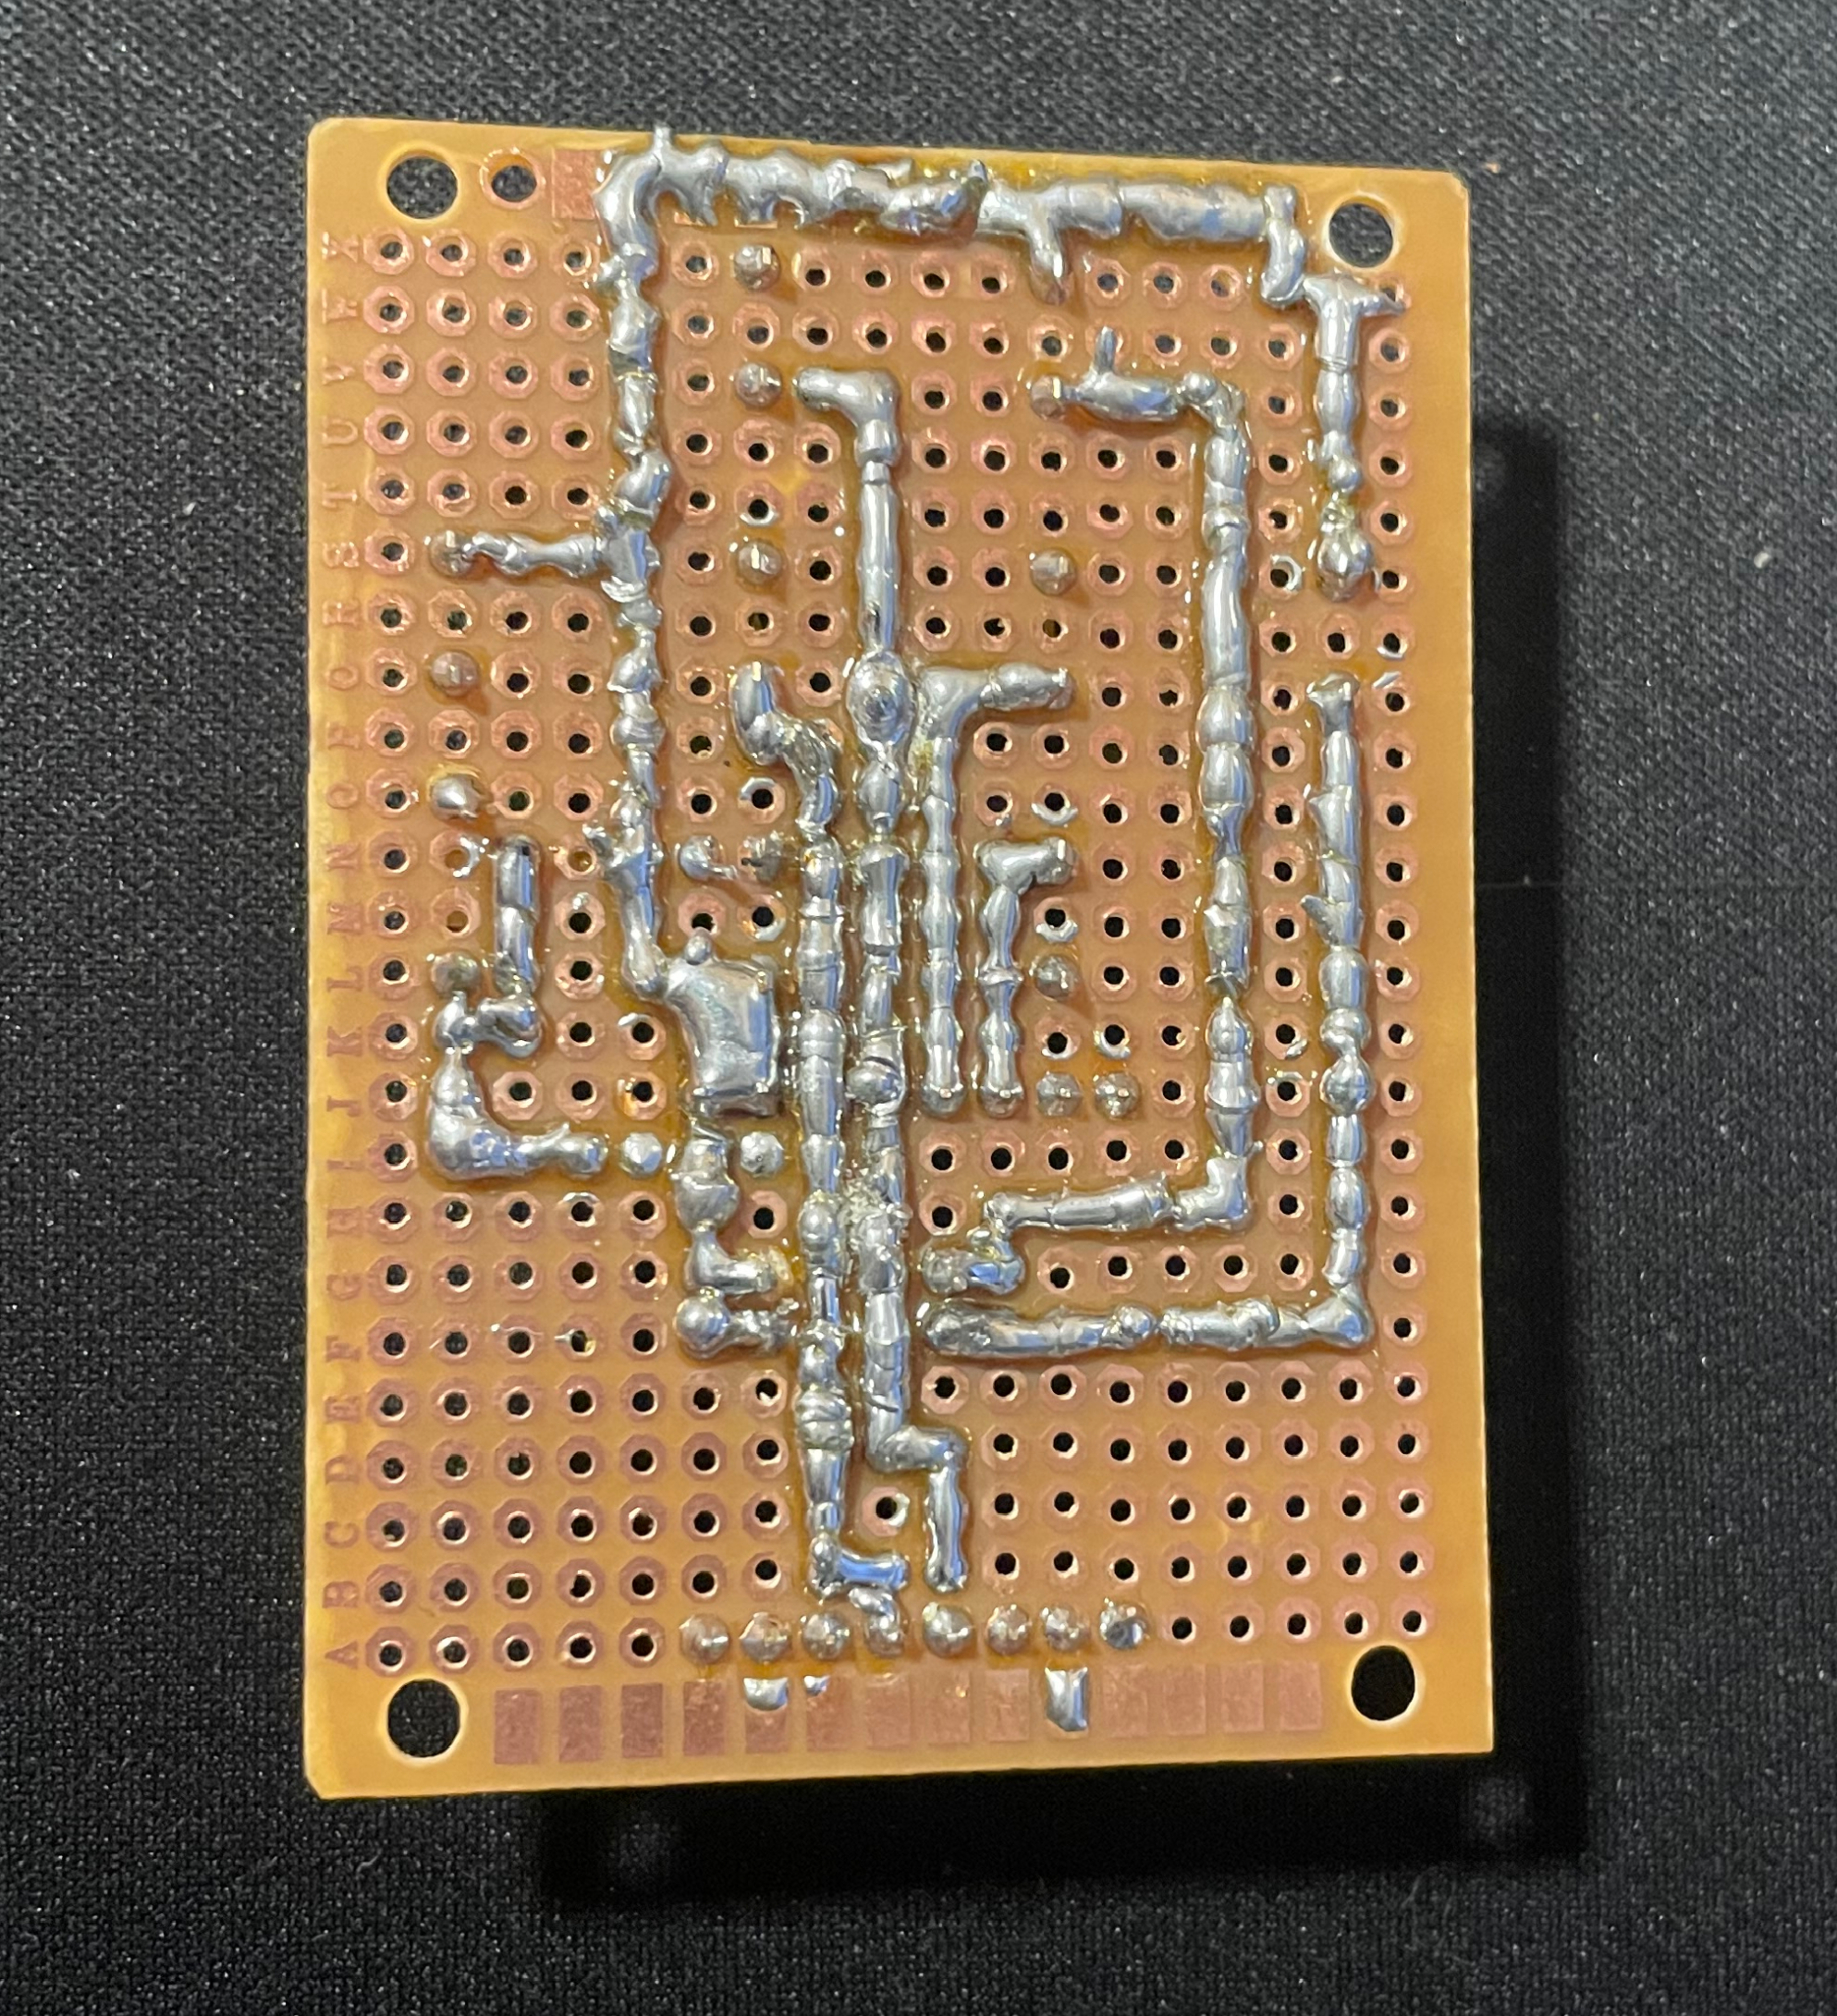
\includegraphics[width=0.4\linewidth]{image/zapajeni.PNG}
     \caption{Ručně pájená deska s plošnými spoji }
     \label{fig:placeholder}
 \end{figure}

\subsection{Využitý hardware pro ovladač}
\begin{itemize}
    \item \textbf{4× mikrospínač}
    \item \textbf{1× ESP8266}
    \item \textbf{4× 10 k\(\Omega\) rezistor}
    \item \textbf{2× \textbf{female header} (8 pinů)}
\end{itemize}
\newpage

\section{Hardware autíčka}
\label{sec:auticko}

Pro konstrukci autíčka byl zvolen jednoduchý a spolehlivý hardware, který umožňuje snadné řízení i případné rozšiřování projektu. Bezdrátový přijímač ES2866 \ref{esp}poskytuje stabilní komunikaci mezi ovladačem a vozidlem, což je klíčové pro přesné reakce při jízdě. H‑můstek L9110S byl vybrán díky své kompaktnosti, nízké ceně a schopnosti efektivně řídit dva stejnosměrné motorky nezávisle na sobě. Použité DC motorky jsou lehké, energeticky nenáročné a ideální pro malé mobilní platformy, kde je důležitá jednoduchost zapojení i dostatečný výkon pro pohyb. Všechny tyto části mám propůjčené od pana učitele Mgr. Marcela Godovského.

\subsection{Výhody zapojení}
Použité zapojení přijímače (receiver) přináší přehlednou a logickou strukturu celého systému. Mikrokontrolér ESP8266 přijímá řídicí data z ovladače a na jejich základě přímo ovládá H-můstek, který řídí chod motorů. Toto řešení minimalizuje zpoždění mezi přijetím povelu a reakcí vozidla, což je důležité pro plynulé ovládání. Další výhodou je modularita zapojení, kdy lze jednotlivé části systému snadno upravit nebo rozšířit bez nutnosti zásadních změn v celé konstrukci. Zapojení je také nenáročné na počet součástek, čímž se snižuje riziko poruch a zjednodušuje údržba.
\subsection{Nevýhody zapojení}
Nevýhodou zvoleného řešení je omezený výkon použitého H-můstku L9110S, který není vhodný pro výkonnější motory nebo vyšší zatížení. To omezuje možnosti dalšího rozšíření projektu, například o těžší konstrukci nebo vyšší rychlost vozidla. Dalším omezením je absence zpětné vazby z motorů, což znamená, že systém nedokáže sledovat skutečnou rychlost nebo zatížení pohonu. Řízení vozidla je tedy založeno pouze na přijatých povelích bez další kontroly, což může mít negativní vliv na přesnost pohybu v náročnějších podmínkách.
\newpage
\subsection{Napajení}
Napájení celého systému je řešeno pomocí čtyř AA baterií zapojených do série. Toto zapojení poskytuje napětí přibližně 6 V, které je vhodné pro napájení použitých DC motorů i dalších elektronických součástí. Zvolené řešení bylo vybráno především pro svou jednoduchost, snadnou dostupnost baterií a možnost rychlé výměny bez nutnosti použití externího napájecího zdroje.

Napájecí napětí je dále distribuováno k jednotlivým částem systému, přičemž mikrokontrolér ESP8266 je napájen přes svůj integrovaný stabilizátor, který zajišťuje požadované provozní napětí. Motory jsou napájeny přímo z bateriového zdroje prostřednictvím H-můstku L9110S, což umožňuje efektivní přenos energie a dostatečný výkon pro pohyb vozidla.
\subsection{Schema zapojení}
\begin{figure}[H]
    \centering
    \includegraphics[width=0.75\linewidth]{image/schemaR.png}
    \caption{Schema autička}
    \label{fig:placeholder}
\end{figure}


\chapter{3D modelování krabičky}

\section{3D software}


Při výběru modelovacího softwaru pro můj projekt jsem měl na výběr mezi několika
možnostmi, mezi nimiž byly klíčovými kandidáty Onshape, Sketchfab a Autodesk Inventor.
Po důkladném zvážení všech faktorů jsem se rozhodl pro Autodesk Inventor.

\subsection{Výhody Autodesk Inventoru}
Rozhodl jsem se využít Autodesk Inventor díky mé předchozí zkušenosti s tímto programem.
Tato volba mi umožnila efektivní modelování bez nutnosti učení se nového softwaru.
Díky studentské licenci poskytnuté školou jsem nemusel platit za software.
Autodesk Inventor, specializovaný na inženýrství a konstrukci, odpovídá potřebám mého
projektu díky parametrickému modelování a vhodným nástrojům.
I když může být v uměleckém modelování omezený ve srovnání s některými ostatními
softwary, pro mé konkrétní potřeby a s ohledem na rychlý a efektivní postup modelování
s minimální časovou investicí byla tato volba vhodná a optimální.

\section{3D modely}
Pro konstrukci krabičky bylo nutné vymodelovat dva samostatné 3D modely – spodní část a
horní víko. Spodní díl slouží jako nosná část krabičky a je navržen tak, aby poskytoval
dostatečný prostor pro umístění elektronických komponent a jejich upevnění.
Horní díl krabičky je navržen jako odnímatelné víko, které obsahuje otvory pro ovládací
prvky a díry pro přichycení. Rozdělení krabičky na dva samostatné modely usnadňuje jak
samotnou montáž elektroniky, tak i výrobu pomocí 3D tisku a případnou údržbu zařízení.

Při modelování krabičky byly využity základní nástroje programu Autodesk 
Inventor, zejména náčrt (Sketch), vysunutí (Extrude), odebrání materiálu (Cut) a 
zaoblení hran (Fillet). Model byl vytvářen parametricky, což umožňuje snadnou
úpravu rozměrů krabičky v případě změny velikosti nebo typu použitých 
elektronických komponent.
\newpage
Rozměry krabičky a rozmístění otvorů byly navrženy s ohledem na konkrétní elektronické
součástky použité v projektu. Ovládací prvky jsou umístěny v horním víku tak, aby byly
snadno přístupné při běžném používání ovladače, zatímco vnitřní prostor spodního dílu
zajišťuje bezpečné uložení desky s mikrokontrolérem a propojení vodičů.

Horní a spodní díl krabičky jsou spojeny pomocí šroubů, které zajišťují pevné uchycení
a zároveň umožňují snadné rozebrání krabičky v případě potřeby údržby, opravy nebo
budoucích úprav zapojení.

Model krabičky byl navržen s ohledem na následnou výrobu pomocí 3D tisku. Byly
zohledněny minimální tloušťky stěn, orientace tisku a omezení tiskového procesu, aby
byla zajištěna dostatečná pevnost a funkčnost výsledného výrobku. Výsledný 3D model
krabičky je znázorněn na obrázku \ref{fig:krabicka}.

\begin{figure}[H]
    \centering
    \includegraphics[width=0.5\linewidth]{image/sestava.png}
    \caption{Model krabičky}
    \label{fig:krabicka}
\end{figure}

\newpage
\chapter{Software}
\section{Bezdrátová komunikace ESP-NOW}

ESP-NOW ~\cite{espnow}je bezdrátový komunikační protokol vyvinutý společností Espressif Systems pro mikrokontroléry řady ESP32 a ESP8266. Tento protokol umožňuje výměnu dat mezi zařízeními bez použití klasické Wi-Fi sítě nebo přístupového bodu, čímž se dosahuje nízké latence a malé režie komunikace. Využívá přímou peer-to-peer komunikaci pomocí MAC adres jednotlivých zařízení a je plně podporován v prostředí Arduino IDE. 

\subsection{Princip funkce}

ESP-NOW funguje jako bezspojový (connectionless) protokol, kde zařízení komunikují přímo mezi sebou bez navazování tradičního Wi-Fi spojení. Data jsou odesílána ve formě krátkých paketů s maximální délkou až 250 bajtů. Protokol podporuje různé režimy komunikace:
\begin{itemize}
    \item komunikace jeden-na-jeden,
    \item jeden-na-více (broadcast),
    \item více-na-jeden. 
\end{itemize}
ESP-NOW může pracovat současně s Wi-Fi, pokud je zařízení ve správném režimu, což umožňuje kombinovat rychlou bezdrátovou komunikaci s přístupem do sítě. :contentReference[oaicite:1]{index=1}

\subsection{Výhody}

Mezi hlavní výhody ESP-NOW patří:
\begin{itemize}
    \item velmi nízká latence a režie při přenosu dat,
    \item nízká spotřeba energie ve srovnání s plnohodnotnou Wi-Fi sítí,
    \item možnost šifrování přenášených paketů pro větší bezpečnost,

\end{itemize}
ESP-NOW je ideální pro projekty vyžadující rychlou výměnu malých datových bloků mezi více zařízeními bez nutnosti centrálního routeru. :contentReference[oaicite:2]{index=2}

\subsection{Omezení}

Protokol má také některá omezení, například:
\begin{itemize}
    \item omezená velikost přenášených dat (maximálně 250 bajtů),
    \item maximální počet zařazených peerů při zabezpečené komunikaci,
    \item kratší dosah ve srovnání s klasickou Wi-Fi sítí při stejném výkonu. 
\end{itemize}
Tyto limity je třeba zohlednit při návrhu systémů, které by vyžadovaly přenos větších objemů dat nebo větší topologickou flexibilitu. :contentReference[oaicite:3]{index=3}

\subsection{Implementace v Arduino IDE}

Pro využití ESP-NOW v prostředí Arduino IDE je potřeba nejprve nainstalovat podporu pro desky ESP8266. Poté lze pomocí knihoven \texttt{esp\_now.h} a \texttt{WiFi.h} \ref{knihovny} nakonfigurovat zařízení jako vysílač, přijímač či obojí. Komunikace probíhá prostřednictvím callback funkcí, které zpracovávají odesílání a příjem dat. Každé zařízení musí být předem spárováno se svými komunikačními protějšky pomocí jejich MAC adresy.

\newpage
\section{Ovladač}
Tato část dokumentace popisuje software pro vysílací jednotku založenou na mikrokontroleru ESP8266. Program je napsán v jazyce C++ a je určen pro vývojové prostředí Arduino IDE. Software zajišťuje čtení stavu čtyř tlačítek a jejich bezdrátový přenos pomocí protokolu ESP-NOW.

\subsection{Použité knihovny}
\label{knihovny}
Na začátku programu jsou zahrnuty potřebné knihovny pro práci s Wi-Fi a ESP-NOW komunikací.

\begin{lstlisting}[style=JavaScript, title={Kód}, caption={Zahrnutí knihoven}]
#include <ESP8266WiFi.h>
#include <espnow.h>
\end{lstlisting}

\subsection{Definice pinů tlačítek}
Tlačítka jsou připojena k GPIO pinům mikrokontroleru. V kódu jsou použity interní pull-up rezistory, proto je logická úroveň LOW považována za stisknuté tlačítko.

\begin{lstlisting}[style=JavaScript, title={Kód}, caption={Definice GPIO pinů tlačítek}]
#define BUTTON1_PIN 14  // D5
#define BUTTON2_PIN 12  // D6
#define BUTTON3_PIN 13  // D7
#define BUTTON4_PIN 4   // D8
\end{lstlisting}
\newpage
\subsection{Datová struktura}
Pro přenos informací o stavu tlačítek je použita struktura, která obsahuje čtyři logické proměnné. Každá proměnná reprezentuje jedno tlačítko.

\begin{lstlisting}[style=JavaScript, title={Kód}, caption={Struktura odesílaných dat}]
typedef struct struct_message {
bool button1;
bool button2;
bool button3;
bool button4;
} struct_message;
\end{lstlisting}

\subsection{Inicializace programu}
Ve funkci \texttt{setup()} je inicializována sériová komunikace, nastaven Wi-Fi režim, GPIO piny a ESP-NOW komunikace. Zařízení je nastaveno do role řídicí jednotky (controller).

\begin{lstlisting}[style=JavaScript, title={Kód}, caption={Inicializace ESP-NOW a pinů}]
void setup() {
Serial.begin(115200);
WiFi.mode(WIFI_STA);

pinMode(BUTTON1_PIN, INPUT_PULLUP);
pinMode(BUTTON2_PIN, INPUT_PULLUP);
pinMode(BUTTON3_PIN, INPUT_PULLUP);
pinMode(BUTTON4_PIN, INPUT_PULLUP);

if (esp_now_init() != 0) {
Serial.println("Chyba inicializace ESP-NOW");
return;
}

esp_now_set_self_role(ESP_NOW_ROLE_CONTROLLER);
esp_now_register_send_cb(OnDataSent);
esp_now_add_peer(broadcastAddress, ESP_NOW_ROLE_SLAVE, 1, NULL, 0);
}
\end{lstlisting}
\newpage
\subsection{Hlavní smyčka programu}
V nekonečné smyčce \texttt{loop()} dochází ke čtení stavu jednotlivých tlačítek, uložení hodnot do struktury a jejich odeslání přijímací jednotce. Pro ladění je stav tlačítek vypisován do sériového monitoru.

\begin{lstlisting}[style=JavaScript, title={Kód}, caption={Čtení tlačítek a odesílání dat}]
void loop() {
myData.button1 = !digitalRead(BUTTON1_PIN);
myData.button2 = !digitalRead(BUTTON2_PIN);
myData.button3 = !digitalRead(BUTTON3_PIN);
myData.button4 = !digitalRead(BUTTON4_PIN);

esp_now_send(broadcastAddress, (uint8_t *)&myData, sizeof(myData));

Serial.print("B1: "); Serial.print(myData.button1);
Serial.print(" | B2: "); Serial.print(myData.button2);
Serial.print(" | B3: "); Serial.print(myData.button3);
Serial.print(" | B4: "); Serial.println(myData.button4);

delay(100);
}
\end{lstlisting}
\newpage
\section{Přijímací jednotka}
Tato část dokumentace popisuje software přijímací jednotky založené na mikrokontroleru ESP8266, která ovládá pohyb vozidla pomocí dvou stejnosměrných motorů. Program je napsán v jazyce C++ a určen pro vývojové prostředí Arduino IDE. Komunikace mezi vysílací a přijímací jednotkou je realizována bezdrátově pomocí protokolu ESP-NOW.

\subsection{Použité knihovny}
Na začátku programu jsou zahrnuty knihovny nezbytné pro práci s Wi-Fi rozhraním a ESP-NOW komunikací.

\begin{lstlisting}[style=JavaScript, title={Kód}, caption={Zahrnutí knihoven}]
#include <ESP8266WiFi.h>
#include <espnow.h>
\end{lstlisting}

\subsection{Datová struktura}
Pro příjem informací o stavu tlačítek je použita struktura shodná se strukturou vysílací jednotky. Jednotlivé logické proměnné reprezentují směrová tlačítka ovladače.

\begin{lstlisting}[style=JavaScript, title={Kód}, caption={Struktura přijímaných dat}]
typedef struct struct_message {
  bool button1; // vlevo
  bool button2; // vpřed
  bool button3; // vpravo
  bool button4; // vzad
} struct_message;

struct_message myData;
\end{lstlisting}
\newpage
\subsection{Definice pinů motorů}
Vozidlo je poháněno dvěma stejnosměrnými motory (pravý a levý), které jsou řízeny pomocí PWM signálů. Každý motor má dva řídicí piny pro změnu směru otáčení.

\begin{lstlisting}[style=JavaScript, title={Kód}, caption={Definice GPIO pinů motorů}]
// Pravý motor
#define A1_A 14  // vpřed
#define A1_B 12  // vzad

// Levý motor
#define B1_A 4   // vzad
#define B1_B 5   // vpřed
\end{lstlisting}

\subsection{Řízení rychlosti motorů}
Rychlost motorů je řízena pomocí PWM signálu. Pro přímý pohyb je použita vyšší hodnota rychlosti, zatímco při zatáčení je jeden z motorů zpomalen.

\begin{lstlisting}[style=JavaScript, title={Kód}, caption={Nastavení rychlostí}]
const int speed = 600;
const int turnSpeed = 200;
\end{lstlisting}

Pro zjednodušení řízení motorů je vytvořena pomocná funkce, která nastavuje PWM hodnoty jednotlivých pinů.

\begin{lstlisting}[style=JavaScript, title={Kód}, caption={Funkce pro ovládání motorů}]
void setMotorsPWM(int a1a, int a1b, int b1a, int b1b) {
  analogWrite(A1_A, a1a);
  analogWrite(A1_B, a1b);
  analogWrite(B1_A, b1a);
  analogWrite(B1_B, b1b);
}
\end{lstlisting}
\newpage
\subsection{Příjem dat pomocí ESP-NOW}
Příjem dat z vysílací jednotky je zajištěn pomocí callback funkce, která je automaticky volána při přijetí zprávy. Data jsou zkopírována do struktury a následně vyhodnocena.

\begin{lstlisting}[style=JavaScript, title={Kód}, caption={Callback funkce pro příjem dat}]
void OnDataRecv(uint8_t *mac, uint8_t *incomingData, uint8_t len) {
  memcpy(&myData, incomingData, sizeof(myData));
  lastRecvTime = millis();
  dataReceived = true;
  ...
}
\end{lstlisting}

\subsection{Logika ovládání vozidla}
Na základě kombinací stisknutých tlačítek je určován směr a způsob pohybu vozidla. Program podporuje:
\begin{itemize}
  \item přímý pohyb vpřed a vzad,
  \item zatáčení na místě,
  \item plynulé zatáčení v oblouku,
  \item bezpečnostní zastavení při stisku tří a více tlačítek.
\end{itemize}

Pokud nejsou přijímána žádná data nebo dojde ke ztrátě signálu, vozidlo se automaticky zastaví.
\newpage
\subsection{Inicializace programu}
Ve funkci \texttt{setup()} je inicializována sériová komunikace, nastaven Wi-Fi režim, nakonfigurovány výstupní piny motorů a spuštěna ESP-NOW komunikace v režimu přijímací jednotky (slave).

\begin{lstlisting}[style=JavaScript, title={Kód}, caption={Inicializace přijímací jednotky}]
void setup() {
  Serial.begin(115200);
  WiFi.mode(WIFI_STA);

  pinMode(A1_A, OUTPUT);
  pinMode(A1_B, OUTPUT);
  pinMode(B1_A, OUTPUT);
  pinMode(B1_B, OUTPUT);

  setMotorsPWM(0, 0, 0, 0);

  esp_now_init();
  esp_now_set_self_role(ESP_NOW_ROLE_SLAVE);
  esp_now_register_recv_cb(OnDataRecv);
}
\end{lstlisting}

\subsection{Hlavní smyčka programu}
V hlavní smyčce \texttt{loop()} je kontrolováno, zda jsou přijímána data. Pokud dojde k překročení časového limitu, motory jsou automaticky zastaveny, což zvyšuje bezpečnost provozu vozidla.

\begin{lstlisting}[style=JavaScript, title={Kód}, caption={Kontrola ztráty signálu}]
void loop() {
  if (!dataReceived || millis() - lastRecvTime > timeout) {
    setMotorsPWM(0, 0, 0, 0);
  }
}
\end{lstlisting}

\chapter*{Závěr}
\addcontentsline{toc}{chapter}{Závěr}

Cílem této závěrečné studijní práce bylo navrhnout a realizovat funkční model autíčka na dálkové ovládání s využitím mikrokontrolérů ESP8266 a bezdrátové komunikace pomocí protokolu ESP-NOW. Tento cíl byl úspěšně splněn – vznikl kompletní systém skládající se z ovladače a přijímací jednotky, které spolu spolehlivě komunikují a umožňují ovládání pohybu vozidla v reálném čase.

V průběhu práce jsem se seznámil s návrhem hardwaru i softwaru embedded systémů. Naučil jsem se pracovat s mikrokontrolérem ESP8266, navrhovat schémata zapojení a implementaci bezdrátové komunikace bez použití klasické Wi-Fi sítě. Zajímavou zkušeností bylo také řešení omezení hardwaru, například malého počtu analogových vstupů, což vedlo k úpravě původního návrhu ovládání.

Závěrem lze říci, že projekt splnil stanovené cíle a poskytl mi cenné praktické zkušenosti v oblasti elektroniky, programování a bezdrátové komunikace. Získané znalosti považuji za dobrý základ pro další studium i budoucí projekty v oblasti informačních technologií a embedded systémů.

	%% literatura
	\begin{thebibliography}{99}
        \bibitem{espnow}
        „Getting Started with ESP-NOW (ESP8266 with Arduino IDE)“, Random Nerd Tutorials, dostupné z: \url{https://randomnerdtutorials.com/esp-now-esp32-arduino-ide/}.
       \bibitem{pinout}
            „ESP8266 Pinout Reference: Which GPIO Pins Should You Use?“, Random Nerd Tutorials,  
            dostupné z: \url{https://randomnerdtutorials.com/esp8266-pinout-reference-gpios/}

	\end{thebibliography}
	
	%% obrázky 
	\listoffigures
	
	%% tabulky
	\listoftables
	
	\appendix %% začínají přílohy
	
	\titleformat{\chapter}[block]{\scshape\bfseries\LARGE}{Příloha \thechapter}{10pt}{\vspace{0pt}}[\vspace{-22pt}] %% nastavení nadpisu u příloh
	
	

	
	
\end{document}